\documentclass[border=5pt]{standalone}
\usepackage{tikz}
\usepackage{amsmath}
\usetikzlibrary{calc, positioning, arrows.meta, 3d}
\begin{document}
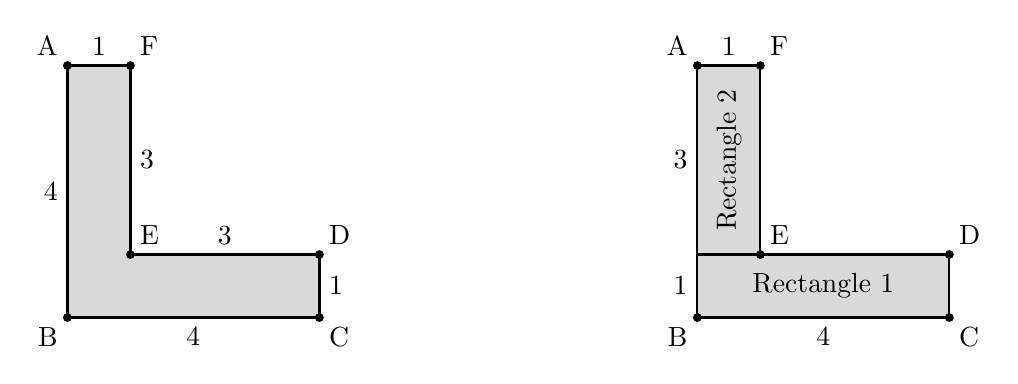
\begin{tikzpicture}[scale=0.8]
% Left figure - Pure L-shape
\begin{scope}[xshift=-5cm]
\draw[thick, fill=gray!30] (0,0)--(4,0)--(4,1)--(1,1)--(1,4)--(0,4)--cycle;

\fill (0,0) circle (2pt) node[below left] {B};
\fill (4,0) circle (2pt) node[below right] {C};
\fill (0,4) circle (2pt) node[above left] {A};
\fill (4,1) circle (2pt) node[above right] {D};
\fill (1,1) circle (2pt) node[above right] {E};
\fill (1,4) circle (2pt) node[above right] {F};
% Add dimensions
\node[below] at (2,0) {4};
\node[right] at (4,0.5) {1};
\node[left] at (0,2) {4};
\node[above] at (0.5,4) {1};
\node[right] at (1,2.5) {3};
\node[above] at (2.5,1) {3};
\end{scope}

% Right figure - Decomposed L-shape
\begin{scope}[xshift=5cm]
% Draw L-shape with clear dimensions
\draw[thick, fill=gray!30] (0,0) rectangle (4,1);
\draw[thick, fill=gray!30] (0,1) rectangle (1,4);

\node[below] at (2,0) {4};
\node[left] at (0,0.5) {1};
\node[left] at (0,2.5) {3};
\node[above] at (0.5,4) {1};

% Label the rectangles
\node at (2,0.5) {Rectangle 1};
\node[rotate=90] at (0.5,2.5) {Rectangle 2};

% Mark key points for reference
\fill (0,0) circle (2pt) node[below left] {B};
\fill (4,0) circle (2pt) node[below right] {C};
\fill (0,4) circle (2pt) node[above left] {A};
\fill (4,1) circle (2pt) node[above right] {D};
\fill (1,1) circle (2pt) node[above right] {E};
\fill (1,4) circle (2pt) node[above right] {F};

\end{scope}
\end{tikzpicture}
\end{document}
